\documentclass{article}
\usepackage[utf8]{inputenc}
\usepackage{graphicx}
\usepackage{hyperref}
\usepackage{geometry}
\geometry{a4paper} % Set the page size to A4
\usepackage{listings} % Package for including code in the document

\title{Práctica 07: Funciones en SQL}
\author{Carlos I. Padilla Herrera}
\date{13 de mayo de 2024}

\lstset{frame=single, % Adds a frame around the code
        basicstyle=\small\ttfamily, % Use a small, true type font
        language=SQL, % SQL syntax highlighting
        showstringspaces=false} % Don't mark spaces in strings

\begin{document}

\begin{titlepage}
    \centering
    \vspace*{1cm}
    \Huge\textbf{Curso de base de datos entre semana G0224}
    
    \vspace{0.5cm}
    \LARGE Escuela de Código PILARES
    
    \vspace{1.5cm}
    \textbf{Carlos Ignacio Padilla Herrera}
    
    \vspace{2cm}
    \Large\textbf{Folio:} 794DR02
    
    \vspace{0.5cm}
    \Large\textbf{Práctica 09:} Operaciones en una base de datos.
    
    \vfill
    
    \Large\textbf{Fecha:} 13 de mayo de 2024.
    
    \vspace{0.8cm}
\end{titlepage}

\newpage

\section*{Código SQL para la creación de tablas y inserción de datos}

\begin{lstlisting}
-- Creating tables
create table manufacturer (
    code int(10) primary key,
    name varchar(100)
);

create table product (
    code int(10) primary key,
    name varchar(100),
    price double,
    manufacturer_code int(10),
    foreign key (manufacturer_code) references manufacturer(code)
);

-- Inserting manufacturers
insert into manufacturer (code, name) values
(1, 'Asus'),
(2, 'Lenovo'),
(3, 'Hewlett-Packard'),
(4, 'Samsung'),
(5, 'Seagate'),
(6, 'Crucial'),
(7, 'Gigabyte'),
(8, 'Huawei'),
(9, 'Xiaomi');

-- Inserting products
insert into product (code, name, price, manufacturer_code) values
(1, 'Disco Duro SATA3 1TB', 86.99, 5),
(2, 'Memoria RAM DDR4 8GB', 120, 6),
(3, 'Disco SSD 1TB', 150.99, 4),
(4, 'GeForce GTX 1050 Ti', 185, 7),
(5, 'GeForce GTX 1080 Xtreme', 755, 6),
(6, 'Monitor 24 LED Full HD', 202, 1),
(7, 'Monitor 27 LED Full HD', 245.99, 1),
(8, 'Portatil Yoga 520', 559, 2),
(9, 'Portatil Ideapad 320', 444, 2),
(10, 'Impresora HP Deskjet 3720', 59.99, 3),
(11, 'Impresora HP Laserjet Pro M26nw', 180, 3);
\end{lstlisting}

\newpage % Inicia una nueva página

\section*{1. Lista el nombre de todos los productos que hay en la tabla producto.}


\begin{figure}[ht]
    \centering
    {
        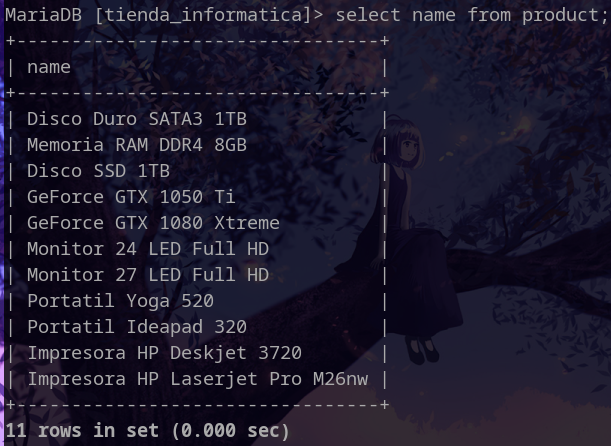
\includegraphics[width=\linewidth]{01screenshot.png} % Asegúrate de que el nombre del archivo y la extensión son correctos
    }
    \caption{Lista de todos los productos que hay en la tabla producto.}
\end{figure}

\newpage % Inicia una nueva página

\section*{2. Lista los nombres y los precios de todos los productos de la tabla producto.}

\begin{figure}[ht]
    \centering
    {
        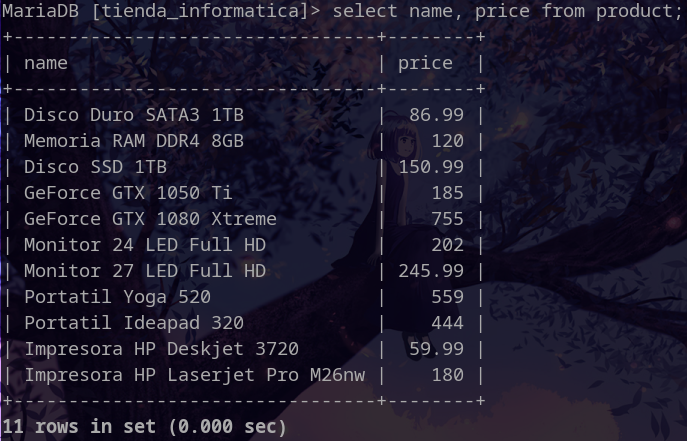
\includegraphics[width=\linewidth]{02screenshot.png} % Asegúrate de que el nombre del archivo y la extensión son correctos
    }
    \caption{Captura de pantalla de los nombres y precios de todos los productos de la tabla producto.}
\end{figure}


\newpage % Inicia una nueva página

\section*{3. Lista todas las columnas de la tabla producto.}

\begin{figure}[ht]
    \centering
    {
        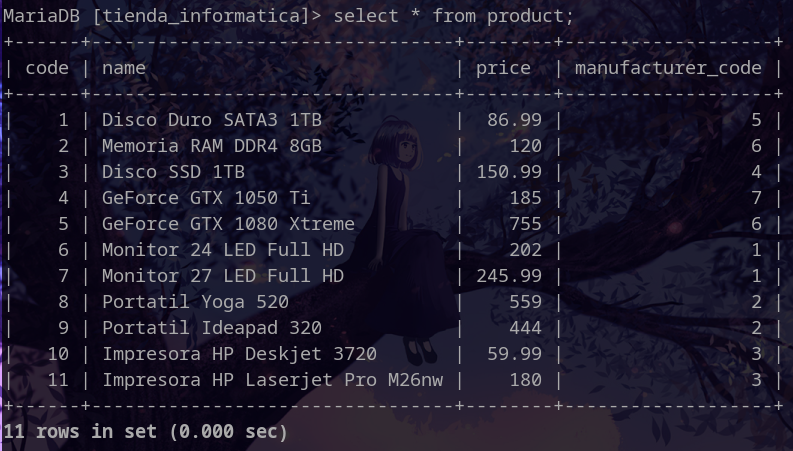
\includegraphics[width=\linewidth]{03screenshot.png} % Asegúrate de que el nombre del archivo y la extensión son correctos
    }
    \caption{Captura de pantalla de las columnas de la tabla producto.}
\end{figure}
\newpage % Inicia una nueva página

\section*{4. Devuelve una lista con el nombre del producto, precio y nombre de fabricante de todos 
los productos de la base de datos.}

\begin{figure}[ht]
    \centering
    {
        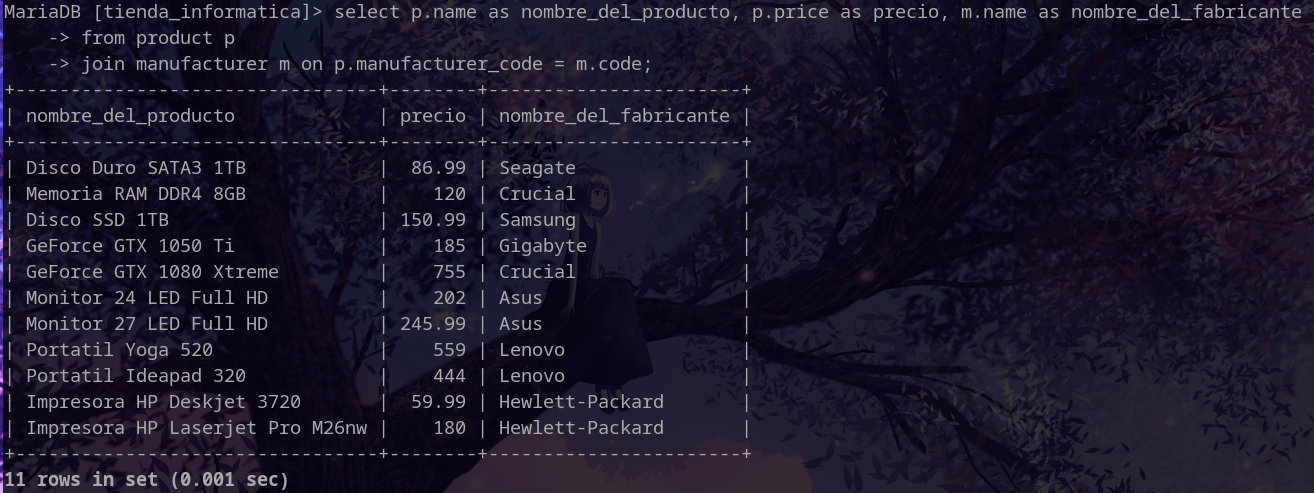
\includegraphics[width=\linewidth]{04screenshot.png} % Asegúrate de que el nombre del archivo y la extensión son correctos
    }
    \caption{Captura de pantalla de una lista de todos los productos de la base de datos.}
\end{figure}
\newpage % Inicia una nueva página

\section*{1. Devuelve todos los productos del fabricante Lenovo. (Sin utilizar INNER JOIN).}

\begin{figure}[ht]
    \centering
    {
        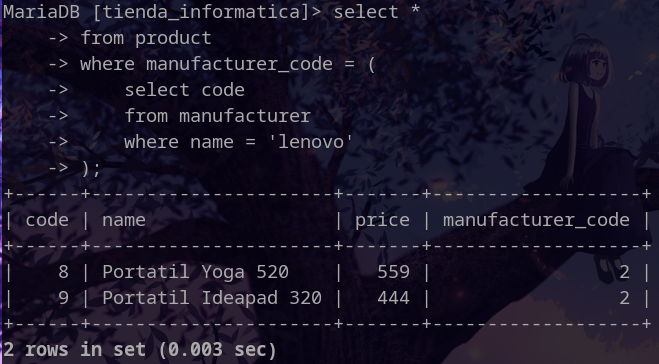
\includegraphics[width=\linewidth]{05screenshot.png} % Asegúrate de que el nombre del archivo y la extensión son correctos
    }
    \caption{Captura de pantalla de todos los productos de Lenovo.}
\end{figure}
\newpage % Inicia una nueva página

\section*{2. Devuelve todos los datos de los productos que tienen el mismo precio que el producto más caro 
del fabricante Lenovo. (Sin utilizar INNER JOIN).}

\begin{figure}[ht]
    \centering
    {
        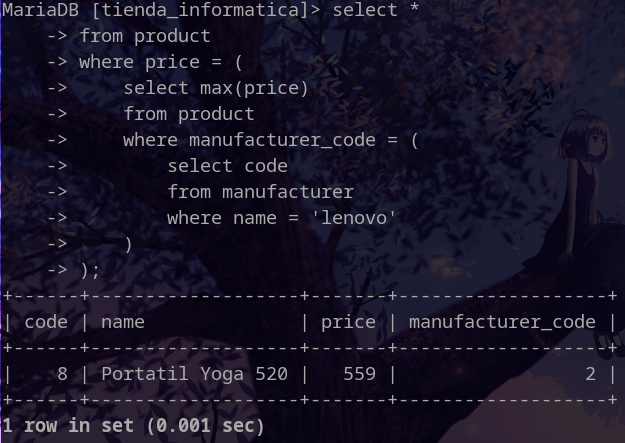
\includegraphics[width=\linewidth]{06screenshot.png} % Asegúrate de que el nombre del archivo y la extensión son correctos
    }
    \caption{Captura de pantalla de los productos que tienen el mismo precio que el producto más caro de Lenovo.}
\end{figure}
\newpage % Inicia una nueva página

\section*{3. Lista el nombre del producto más caro del fabricante Lenovo.}

\begin{figure}[ht]
    \centering
    {
        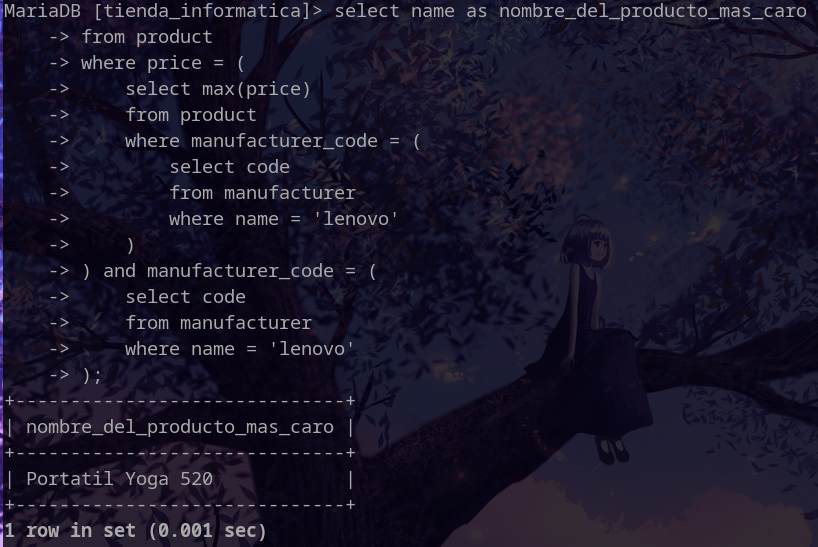
\includegraphics[width=\linewidth]{07screenshot.png} % Asegúrate de que el nombre del archivo y la extensión son correctos
    }
    \caption{Captura de pantalla producto más caro del fabricante Lenovo.}
\end{figure}

\end{document}
